\chapter{Literature Review}\label{chapter:lit_review}
\glsresetall

\section{Overview}
Building on the background presented in Chapter \ref{chapter:background}, this chapter reviews literature directly related to the technical contributions of this thesis. We begin with compositional approaches to \gls{ml}-based \glspl{cps}, distinguishing model-level decomposition from system-level pipeline design and identifying the research gap that motivates our work. We then survey three strands of related work---\gls{fpga} implementation and timing analysis, compositional safety and verification, and compositional explainability---before reviewing the literature on our two case-study domains (autonomous vehicles and personalised mood score prediction). Throughout, we highlight gaps that the subsequent technical chapters address.


\section{Compositional Modelling in ML-based CPS}
\label{sec:lit_compositional_modelling}

A compositional approach, as elaborated in Section \ref{sec:lit_compositionality} of Chapter \ref{chapter:background}, promotes the use of multiple smaller, functionally equivalent subsystems instead of a single, large, monolithic system. This methodology is particularly advantageous for the design of \gls{ml}-based \glspl{cps}, where scalability, modularity, and verifiability are critical concerns. 

Recent research in data-driven \gls{cps} design has explored various strategies to incorporate compositionality. These efforts span a spectrum of objectives and methodologies. For instance, several studies, including \cite{dreossi_compositional_2018, seshia_formal_2018, dreossi_verifai_2019, naik_robustness_2020}, leverage compositional architectures specifically to facilitate the formal verification of \gls{cps}. By structuring systems as compositions of smaller, verifiable modules, these works aim to make the verification process more tractable and scalable, enabling the analysis of properties that would be infeasible to check in a monolithic setting.

While the works mentioned above use the idea of compositionality, they do so on a system level. They do not tackle the monolithic ML model in a compositional or modular manner, accounting for most of the verification overhead due to its nonlinearity and computational complexity. Although \cite{watanabe_modular_2017} and \cite{pan_decomposing_2020} present approaches to decomposing trained monolithic ANNs to multiple small independent networks, their focus is not on easing verification. Hence, the overall network size remains unchanged or may even increase, which can prove detrimental despite the smaller size of the decomposed models. On the other hand, studies, such as \cite{gokulanathan_simplifying_2020} and \cite{elboher_abstraction-based_2020}, which use model reduction techniques to simplify ANNs instead of compositionality, do not always produce a simple ANN, and the method used therein is not always intuitive. 

It is important to distinguish the model-level decomposition discussed above from system-level pipeline composition, which is already common in industrial practice. The autonomous driving domain illustrates this distinction clearly. Waymo's architecture employs a modular, multi-model pipeline in which separate \gls{ann} models handle distinct tasks---perception from LiDAR, camera, and radar inputs, behaviour prediction of other road users, and motion planning---each independently trained and connected in a processing pipeline \cite{sun_scalability_2020, bansal_chauffeurnet_2019}. This represents \emph{system-level composition}: the overall system is decomposed into functional modules, but each module remains a monolithic \gls{ann} that is trained and deployed as a single black box. In contrast, Tesla's Full Self-Driving (FSD) system has historically pursued a more end-to-end approach, using large monolithic neural networks to map raw camera inputs more directly to driving outputs \cite{chen_end--end_2024, tampuu_survey_2022}. More recent iterations of both platforms have converged towards hybrid architectures, but the fundamental dichotomy between modular pipelines and monolithic end-to-end models persists across the industry \cite{chen_end--end_2024}.

Crucially, the compositionality proposed in this thesis is fundamentally different from this system-level pipeline design. Rather than arranging multiple independently trained models in a processing pipeline, our approach concerns the decomposition of a \emph{single} \gls{ann} model---for example, a lane-change classifier---into multiple smaller sub-models (e.g., one binary classifier per class) that collectively replace the original monolithic model. This is \emph{model-level decomposition}. System-level composition, as practised by Waymo and others, does not address the verification, \gls{wcet}, or explainability challenges inherent in each individual monolithic model within the pipeline: each model in a Waymo-style pipeline is still a large, monolithic black box that is difficult to formally verify, implement on resource-constrained hardware, and explain. Model-level decomposition, as developed in this thesis, directly tackles these challenges by reducing the size and complexity of each individual model.

Overall, there is a lack of research that studies how to systematically, quantitatively, and objectively decompose large monolithic ANN models into smaller networks at the model level. Moreover, a detailed quantitative comparison between monolithic and compositional designs based on their performance is long overdue. The remainder of this chapter reviews existing work in the three areas---timing analysis, safety, and explainability---where model-level compositionality offers the greatest benefit, and situates our case studies within that context.


\section{Implementing Compositional ANN Models to FPGA Hardware for Timing Analysis}
\label{sec:lit_fpga_implementation}



\begin{table}[htbp]
  \caption{Comparison between related works and our hardware compilation method (Mon. for Monolithic design, and Com. for Compositional design. Composed in the Design column stands for designs that combine (not decompose) multiple smaller models.)}
  \begin{tabularx}{6in}{|X|X|X|X|X|X|X|}
  \hline
 Research & Precision & Activation & Activation & Neurons/ & General & Design \\
   & & Approx. & Function & Layers & Method & \\
  \hline
 Himavathi et al.\cite{himavathi_feedforward_2007} & Fixed   & \gls{lut} & Sigmoid, Linear  &23/4 & No & Mon. \\
 Marouf et al. \cite{marouf_fpga_2012} & Floating  & \gls{lut}  & Linear, Sigmoid & 7/2 & No & Mon. \\
 Nguyen et al. \cite{nguyen_efficient_2018} & Fixed    & \gls{lut}  & Relu, Sigmoid & 58/2 & No & Mon.    \\
 Allen et al. \cite{allen_compositional_2019-1} & Fixed    & \gls{lut}  & Relu, Sigmoid, \gls{tanh}, Linear & 35/6 & Yes & Composed  \\
 Sarić et al. \cite{saric_fpga-based_2020-1} & Fixed  & \gls{lut}  & Sigmoid & 15/2& No    & Mon. \\
 Zairi et al. \cite{zairi_fpga-based_2020} & Fixed   & \gls{lut} & \gls{tanh}, Sigmoid & 7/2 & No & Mon. \\
  \hline
  \end{tabularx}
  \label{tab:fpga_comparison}
\end{table}


Timing analysis for worst-case execution time (WCET) is a critical component in the design of time-critical cyber-physical systems (CPS). By verifying that every computation finishes within its allotted budget, we can guarantee the system meets stringent real-time requirements. Notably, implementing neural networks on dedicated FPGA hardware simplifies this analysis: the absence of caches, pipelines, branch predictors, and out-of-order execution yields fully predictable, cycle-accurate behaviour \cite{wilhelm_worst-case_2008}.  

To understand how these benefits have been exploited, we survey existing works that deploy artificial neural network (ANN) models on FPGAs. Table \ref{tab:fpga_comparison} summarises each approach in terms of numerical precision, activation-function approximation method, supported activation functions, tested network size (neurons and layers), application specificity, and support for compositional designs.  

From this comparison, several trends and limitations emerge. First, most hardware compilation techniques are tailored to particular applications and validated only on small-scale networks. The key obstacle appears to be the heavy resource demands of large ANNs on affordable FPGA platforms, which discourages general-purpose, scalable solutions. Second, nearly all approaches approximate activation functions using lookup tables (LUTs), and typically cover only a few activation functions, e.g.\ Sigmoid, \gls{tanh}, or \gls{relu}, while more complex functions like Softmax (which requires exponentials) remain unsupported.  

Finally, despite the clear advantages of synchronous hardware semantics for deterministic timing, few works adopt a truly synchronous execution model (see Section \ref{sec:real_time_syn} in Chapter \ref{chapter:background}). \cite{allen_compositional_2019} and \cite{yang_compositional_2020} do employ synchronous hardware for multiple smaller ANNs, but neither addresses compositional implementation of a single, larger ANN, nor extends to a broad class of activation functions. In fact, no existing approach both decomposes monolithic ANN models into compositional architectures and implements them on FPGAs with formal timing analysis in mind.

Taken together, the evidence from existing hardware implementations reinforces three interconnected requirements that motivate this thesis. First, \glspl{fpga} are not merely an alternative to embedded \glspl{gpu}; they are a viable platform for obtaining provable \gls{wcet} bounds on \gls{ann} inference. As Wilhelm et al.\ \cite{wilhelm_worst-case_2008} establish, static \gls{wcet} analysis depends on fully deterministic hardware behaviour---a property that \glspl{gpu}, with their caches, dynamic thread scheduling, and shared-memory contention, fundamentally cannot provide. For safety-critical \glspl{cps} that must comply with certification standards, measurement-based timing estimates are insufficient; only the cycle-accurate, cache-free execution model of \glspl{fpga} enables the formal timing guarantees required.

Second, the compilation of \gls{ann} models to synthesisable VHDL is a necessary step in this verification chain. Python-based training frameworks such as TensorFlow \cite{martin_abadi_tensorflow_2015} and PyTorch \cite{paszke_pytorch_2019} produce software-level model descriptions that cannot be directly executed on \gls{fpga} fabric in a timing-analysable manner. A systematic compilation to VHDL bridges this gap: it translates the trained model's weights, biases, and activation functions into a synchronous hardware description whose execution time is bounded by a fixed number of clock cycles. Without such a compiler, practitioners are forced to hand-craft hardware designs for each network topology---a process that, as Table \ref{tab:fpga_comparison} shows, has limited existing implementations to at most 58~neurons and a narrow set of activation functions. An automated VHDL compilation pathway is therefore essential for scaling \gls{fpga}-based \gls{ann} deployment beyond small, application-specific prototypes.

Third, compositional decomposition directly addresses the resource constraints that have restricted existing \gls{fpga} implementations to small networks. Monolithic \glspl{ann} demand proportionally large amounts of \gls{fpga} logic resources, on-chip memory, and routing fabric---requirements that quickly exceed the capacity of affordable \gls{fpga} devices \cite{saric_fpga-based_2020-1, nguyen_efficient_2018}. By decomposing a single large model into multiple smaller sub-models, compositionality reduces the peak resource demand of any individual component, enables the sub-models to be mapped to separate hardware resources for true parallel execution, and makes \gls{wcet} analysis tractable for each sub-model independently. The synchronous frameworks of Allen et al.\ \cite{allen_compositional_2019} and Yang et al.\ \cite{yang_compositional_2020} demonstrate the feasibility of running multiple smaller \glspl{ann} on a single \gls{fpga}, but neither addresses the prior step of \emph{deriving} those sub-models from a monolithic original---the gap that this thesis fills.


\section{Safe-by-Construction Compositional CPS}
\label{sec:lit_safe_compositional}

Formal verification of \glspl{cps} is a challenging task, especially for large-scale CPSs. This complexity is exacerbated by the use of ML-based components, such as \glspl{ann}, in the system, which have large state spaces and are nonlinear. Table \ref{tab:included-studies-short} shows some of the current works on verifying \gls{ann}-based \glspl{cps}.


\begin{table}[htbp]
  \centering
  \caption{Studies that perform verification of ANN-based CPSs}
  \label{tab:included-studies-short}
  \begin{tabular}{|p{4cm}|p{6cm}|p{4cm}|}
  \hline
  \textbf{Study} & \textbf{Focus} & \textbf{Verification Paradigm} \\ \hline
  
 Ivanov et al.\ (2021) \cite{ivanov_compositional_2021} & Compositional verification of \gls{ann} controllers & Reachability analysis \\ \hline
  
 Watson et al.\ (2025) \cite{Watson2025Scenario} & Scenario-based verification with neural perception & Probabilistic, scenario-based \\ \hline

 Zhou et al.\ (2023) \cite{Zhou2023Compositional} & Invariant-based verification of \gls{ann}-controlled systems & Inductive invariants \\ \hline
  
 Ivanov et al.\ (2018) \cite{Ivanov2019Verisig} & Safety verification of hybrid systems with \gls{ann} & Reachability analysis \\ \hline
  
 P\u{a}s\u{a}reanu et al.\ (2018) \cite{pasareanu_compositional_2018} & Compositional verification of \gls{ann} components & Assume-guarantee reasoning \\ \hline
  
 Cai et al.\ (2024) \cite{Cai2024Scalable} & Surrogate verification for image-based controllers & Reachability analysis \\ \hline
  
 Wang et al.\ (2022) \cite{Wang2022Verified} & Temporal logic objectives for \gls{ann} controllers & Automata-based \\ \hline
  
 Elboher et al.\ (2019) \cite{Elboher2020Abstraction} & Abstraction framework for \gls{ann} verification & Abstraction-based \\ \hline
  
 Paulsen et al.\ (2020) \cite{Paulsen2020ReluDiff} & Differential verification of \gls{ann}s & Symbolic intervals \\ \hline
  
 Kouvaros et al.\ (2021) \cite{Kouvaros2021Towards} & Scalable ReLU network verification & \gls{mip} reduction \\ \hline
  
  \end{tabular}
  \end{table}

  
The literature on verification of neural-network-enabled systems can be grouped into three broad areas. First, a core set of works directly embraces compositional falsification or assume-guarantee reasoning by decomposing a complex controller into manageable subunits \cite{ivanov_compositional_2021, pasareanu_compositional_2018}. \cite{Zhou2023Compositional} extend this theme by using inductive invariants. \cite{Watson2025Scenario} further uses compositionality to get error-bound guarantees under stochastic conditions. A second area centres on reachability, hybrid-system methods \cite{Ivanov2019Verisig, Kouvaros2021Towards} and surrogate verification \cite{Cai2024Scalable, Wang2022Verified}. Techniques such as abstraction-refinement loops \cite{Elboher2020Abstraction} and differential verification via symbolic-interval analysis \cite{Paulsen2020ReluDiff} provide complementary means to bound and compare network behaviours. Finally, informal orthogonal techniques, such as adversarial training \cite{10.1145/3134599}, have also been used to make ML models safer by increasing their robustness against certain unexpected inputs and scenarios.


However, these compositional and reachability-based verification methods exhibit NP-complete complexity, resulting in state-space explosion and scalability barriers even with heuristics or advanced branching strategies \cite{pasareanu_compositional_2018, Cai2024Scalable, Kouvaros2021Towards}. Decidability is often confined to shallow architectures—e.g., single hidden-layer networks—while over-approximation techniques trade termination guarantees for coarse abstractions and incomplete proofs \cite{Ivanov2019Verisig, Wang2022Verified}. Moreover, most approaches are tailored to specific network classes or narrow input domains, such as feed-forward ReLU models or discretised scenarios, which limits their generality and precision \cite{Paulsen2020ReluDiff, Watson2025Scenario}. Achieving tighter error bounds invariably increases computation and memory costs, leading to timeouts or looser probabilistic guarantees when refinements or scenario counts are constrained \cite{Zhou2023Compositional, Watson2025Scenario}. Finally, adversarial training does not provide any formal guarantees on model behaviour.

Consequently, there are other bodies of work for verification, which are dynamic and lightweight. For example, Runtime Verification and Runtime Enforcement. We do not need to model the system here. We just take the executions of the (black-box ANN/ML) systems at runtime and monitor them to ensure their compliance with a set of formal requirements. Additionally, in the event of a violation, using an enforcement monitor/enforcer corrects the output. This means an (untrustworthy) input execution (in the form of a sequence of events that does not comply with the policy) is modified into an output sequence that complies with a policy (e.g., a safety requirement). 


There are several mechanisms by which a correction is made: framework \cite{10.1145/353323.353382} considers blocking the execution in case of a violation,  \cite{10.1007/s10207-004-0046-8} considers modifying input sequence by suppressing and/or inserting actions, \cite{10.1007/s10703-014-0215-y} considers buffering input actions until a future time when it could be forwarded, \cite{10.1145/3092282.3092291,pearce_smart_2020} considers instantly correcting the executions suitable for reactive systems, safety-critical systems and cyber-physical systems. Nevertheless, Runtime Verification and Runtime Enforcement have not been used on compositional ML models.


The need for compositional \gls{ml} design in the safety domain is further underscored by a fundamental scalability argument. As Katz et al.\ \cite{katz_reluplex_2017} have shown, verifying even basic properties of \gls{relu} networks is NP-complete, and the verification cost grows exponentially with the number of neurons and layers. Compositional decomposition directly mitigates this: by replacing a single large model with multiple smaller sub-models, the state space that any individual verification tool must explore is reduced, making component-level verification feasible where monolithic verification would time out \cite{pasareanu_compositional_2018, Kouvaros2021Towards}. 

Furthermore, compositional design can create natural boundaries for runtime enforcement. Rather than enforcing a single global safety property over the aggregate output of a monolithic model, each sub-model can be paired with a dedicated enforcer \cite{10.1145/3092282.3092291, pearce_smart_2020} that monitors compliance with a local sub-policy. This per-component enforcement reduces the state space of each individual monitor, increases the precision of corrective actions, and ensures that a violation in one component can be isolated and corrected without disrupting the outputs of other components. 

The compositional structure should also enable policy mining at the sub-model level: safety properties can be extracted from the training data of each component independently, yielding tighter and more meaningful constraints than those obtainable from a monolithic model whose features span multiple, unrelated domains.

All in all, while there have been attempts to develop safer ML-based systems using compositionality and other approaches, there have been little to no attempts to develop a formal framework that combines formalism with compositional ML model design to make ML-based systems safe by construction, i.e., formal safety is designed into every stage of ML-based system design. 


\section{Compositionality for Designing Explainable Systems}
\label{sec:lit_explainability}

Often, in some systems, especially ones used in the healthcare domain, predicting with high accuracy is insufficient. Most \gls{ml} approaches are black-box approaches, i.e., they do not show how they reached a prediction \cite{molnar_interpretable_nodate}. Without explaining why a model predicts, professionals using such models cannot determine what insights the prediction contains \cite{joyce_explainable_2023}. These insights can then be used to check a model's fidelity (whether the model predictions make sense) \cite{kamath_introduction_2021} and suggest solutions based on these explanations. This ensures the transparency and accountability of the models. 

Recent advances in \gls{xai} offer solutions to the problem of trustworthiness in ML models. Explainable models, such as Decision Trees \cite{molnar_interpretable_nodate}, can be easily processed/simplified to explain their outputs \cite{barredo_arrieta_explainable_2020}. However, their expressive power is limited by their size, and increasing their expressiveness decreases their interpretability. ANN models can make more complex associations from multimodal data and yield better-performing models \cite{goodfellow_deep_2016,joyce_explainable_2023}, but are not inherently explainable \cite{molnar_interpretable_nodate}. 

With the availability of post-hoc explainable methods (see Section \ref{sec:intro_explainability} in Chapter \ref{chapter:background} for a deeper dive into these methods), such as Shapley Additive Explanations (SHAP) \cite{lundberg_unified_2017} and Local  Interpretable Model-agnostic Explanations (LIME) \cite{ribeiro_why_2016}, explaining performant black-box DL models has become easier \cite{molnar_interpretable_nodate}. Studies such as \cite{korda_identification_2022, schultebraucks_validated_2020, binder_morphological_2021} use explainability techniques on ML models to obtain insights into the model outputs. Moreover, with the growth of works using ML-based models in healthcare, recent works have begun exploring explainability in the healthcare setting \cite{wang_explainable_2021, zhu_explainable_2023, squires_identifying_2023, zogan_explainable_2022,shah_personalized_2021}. 

However, the use of explainability has been limited to the extraction of the most influential model features/inputs using SHAP or LIME \cite{byeon_advances_2023}. Furthermore, the development of ML models and their use of explainability has been limited to the monolithic ML/DL model— where a single model ingests a vast array of disparate features—making it challenging to decompose model behaviour into intuitive, clinically meaningful explanations due to the complexity and interdependence of inputs. Also, when the model underperforms, it is often challenging to isolate which cluster (or set of features) is causing the issue since they are all entangled in one model.

Compositional \gls{ml} design can offer a principled solution to these explainability limitations. When a monolithic model is decomposed into sub-models, each handling a semantically coherent group of features, explainability methods such as SHAP \cite{lundberg_unified_2017} and LIME \cite{ribeiro_why_2016} can be applied \emph{within} each sub-model, yielding feature attributions that are confined to a single domain and therefore directly interpretable by domain experts. For instance, in a healthcare application, a sub-model responsible for sleep-related features produces SHAP values that a clinician can immediately relate to sleep hygiene recommendations, without the confounding influence of activity or physiological features that would be present in a monolithic model \cite{joyce_explainable_2023, kamath_introduction_2021}. 

Furthermore, compositional architectures naturally support multi-level explanations: at the global level, the relative contributions of entire sub-models reveal which domains are most influential for a given prediction; at the local level, within-component feature attributions provide fine-grained detail. This hierarchical structure aligns with the practical needs of different stakeholders---clinicians require domain-level summaries, while data scientists need feature-level diagnostics---and addresses the monolithic model's inability to provide explanations at varying granularities \cite{molnar_interpretable_nodate, barredo_arrieta_explainable_2020}. 

The compositional approach also simplifies model debugging: when a model underperforms, the modular structure makes it straightforward to identify which sub-model (and therefore which feature domain) is responsible, enabling targeted retraining without disrupting the other components. Despite the possible advantages, a compositional approach to designing and explaining ML models has not been explored in recent studies. 

Having reviewed the general literature on model-level compositional design and its implications for timing, safety, and explainability, we now turn to the application domains in which this thesis evaluates the proposed framework.


\section{Review of Case Study Literature}
\label{sec:lit_case_studies}
We use two main case studies in this work - the first is the case study of an \gls{av}, and the second is the case study of a personalised mood score prediction model for depression. We discuss the existing literature on the case studies, what current research gaps exist, and what compositional design approaches can address.

\subsection{Developing  Models for Autonomous Vehicles}

An  \gls{av} is a vehicle that is capable of sensing its environment and operating with minimal or no human involvement. Autonomous vehicles are also known as self-driving cars, robotic cars, or driverless cars. The technology is a combination of sensors, cameras, radar, and artificial intelligence (AI) to navigate and drive the vehicle. 

One of the key challenges in developing autonomous vehicles is designing models that can accurately interpret the data collected by the sensors and make decisions in real-time. These models must detect and classify objects in the environment, predict the movements of other vehicles and pedestrians, and plan a safe and efficient route to the destination while handling unexpected situations, such as road closures, accidents, or adverse weather conditions. Hence, they represent a safety-critical \gls{cps}.

To simplify the development of autonomous vehicles, studies often divide the tasks performed by the vehicle into smaller sub-tasks  \cite{zheng_recent_2014}. For example, car-following and lane-changing are two common subtasks that are essential for autonomous driving. In this section, we will discuss each of these subtasks in more detail.


\subsubsection{Car Following}
\gls{cf} is the task of maintaining a safe distance between the  \gls{av} and the vehicle in front of it. This is an essential task for autonomous vehicles, as following too closely can lead to accidents, while following too far behind can slow traffic flow. \gls{cf} algorithms use data from the vehicle's sensors to estimate the speed and position of the vehicle in front of it, and then adjust the vehicle's speed and position accordingly. These algorithms need to be able to handle variations in speed, road conditions, and traffic density, and respond quickly to changes in the environment.

While various car-following models have been proposed in the literature, the Intelligent Driver Model (IDM) \cite{treiber1999, PhysRevE.62.1805} is one of the most widely used models. The IDM is a microscopic car-following model that describes the acceleration of a vehicle based on the distance to the vehicle in front of it, the relative speed, and the desired speed of the driver.

The IDM model is given by the following equation:
\begin{equation}
    \frac{dv}{dt} = a \left( 1 - \left( \frac{v}{v_0} \right)^\delta - \left( \frac{s^*}{s} \right)^2 \right)
\end{equation}

where $v$ is the speed of the vehicle, $a$ is the maximum acceleration, $v_0$ is the desired speed, $\delta$ is the acceleration exponent, $s$ is the distance to the vehicle in front, and $s^*$ is the desired minimum distance. The IDM model is used in this work for its simplicity and its ability to include driver preferences in modelling car-following behaviour. More recently, ANN-based \gls{cf} models have also been proposed in the literature, which use \glspl{ann} to learn the relationship between the vehicle's speed and position and the speed and position of the vehicle in front of it \cite{zhang_simultaneous_2019}. 


\subsubsection{Lane Changing}
Lane changing is the task of moving the  \gls{av} from one lane to another. \gls{lc} is necessary when the vehicle needs to overtake another vehicle, merge onto a highway, or exit a highway. Lane changing algorithms use data from the vehicle's sensors to detect other vehicles in adjacent lanes, estimate their speed and position, and determine when it is safe to change lanes. A key challenge in lane changing is predicting the movements of other vehicles and anticipating how they will respond to the  \gls{av}'s actions. 

\gls{dlc} is a subtype of lane changing where the driver has the choice to change lanes \cite{balal_analysis_2014}. In this case, the  \gls{av} must decide whether it is safe and appropriate to change lanes based on the traffic conditions and the driver's preferences. Usually, a \gls{dlc} occurs when the preceding car is moving slower than the driver's desired speed. Mandatory lane changing, on the other hand, is when the driver is required to change lanes, such as when a lane is closed or when the vehicle needs to exit the highway. In this case, the  \gls{av} must change lanes quickly and safely to comply with the traffic rules or destination requirements (see Figure \ref{fig:car_placement_lit}).

\begin{figure}[htbp]
  \centering
  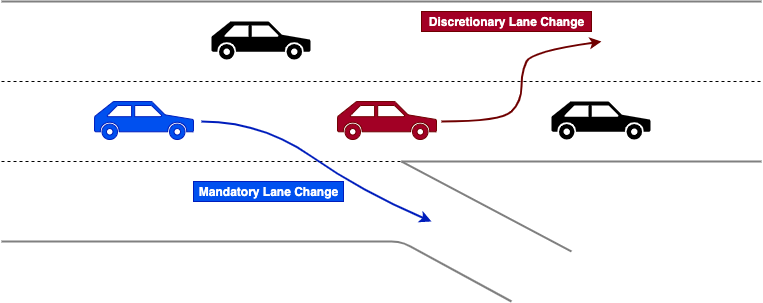
\includegraphics[width=\textwidth]{lit_review/fig/Mandatory_DiscretionaryLC.png}
  \caption{Cars performing a discretionary \gls{lc} (left) and a mandatory \gls{lc} (right). }
  \label{fig:car_placement_lit}
\end{figure}

Modern lane changing models are based on Neural Networks, and there are two main variations in the way \gls{ann}-based LC models are developed. The models presented in~\cite{tomar_prediction_2010} and~\cite{zhang_simultaneous_2019} learn the entire LC procedure as a single process, where the models decide when a vehicle can execute a \gls{lc} by changing the position of the vehicle accordingly. In contrast to this approach, studies such as~\cite{xie_data-driven_2019} and~\cite{liu_deep_2019} model \gls{lc} as a two-step process: (1) learning to decide when it's safe to change lane; and (2) learning to execute the decision, and build models for both steps or either. We use this approach in our work as it allows for the segregation of the vital decision-making module from the succeeding execution module, enabling greater and singular focus on the decision-making module.

The autonomous driving domain exemplifies why all three pillars of this thesis---\gls{fpga}-based timing analysis, compositional safety, and compositional explainability---are needed in concert. The driving subtasks reviewed above are inherently safety-critical and time-critical: a car-following or lane-changing decision must be computed within a strict real-time deadline dictated by vehicle speed and traffic density \cite{zheng_recent_2014}. Monolithic \gls{ann} models for these subtasks cannot be deployed on \glspl{fpga} for formal \gls{wcet} analysis because their size exceeds the resource budgets of affordable devices \cite{saric_fpga-based_2020-1, nguyen_efficient_2018}. Compositional decomposition addresses this directly: by splitting the monolithic model into smaller sub-models---for instance, one binary classifier per lane-change decision class---each sub-model is small enough for \gls{fpga} implementation and synchronous \gls{wcet} analysis \cite{allen_compositional_2019, yang_compositional_2020}. Simultaneously, the decomposition enables per-component safety enforcement \cite{10.1145/3092282.3092291, pearce_smart_2020} and component-level explainability \cite{lundberg_unified_2017}, allowing each driving subtask to be independently verified, monitored, and explained.


\subsection{Personalised Mood Score Prediction for Depression}

Depression is a disorder involving loss of pleasure or interest in activities for long periods and is associated with sustained mood deterioration \cite{health_uk_classification_2010}. It can affect several aspects of life, including relationships and work. According to the World Health Organisation (WHO) 2023 estimates, 5\% of adults (approximately 300 million) worldwide experience depression, with women 50\% more likely to experience depression than men. It is a significant contributor to the 700,000 suicides every year around the world \cite{noauthor_depressive_nodate}. 

Despite this, more than 75\% of people in low- and middle-income countries receive no treatment due to a lack of investment in mental health, a lack of healthcare professionals and social stigma associated with mental health disorders \cite{noauthor_depressive_nodate}. For those who receive treatment, antidepressant medications are often the first line of treatment. However, they have low effectiveness as only one-third of all patients show symptom remission, as evidenced in large clinical trials \cite{gaynes_what_2009, trivedi_evaluation_2006}. 


\begin{figure}[htbp]
  \centering
  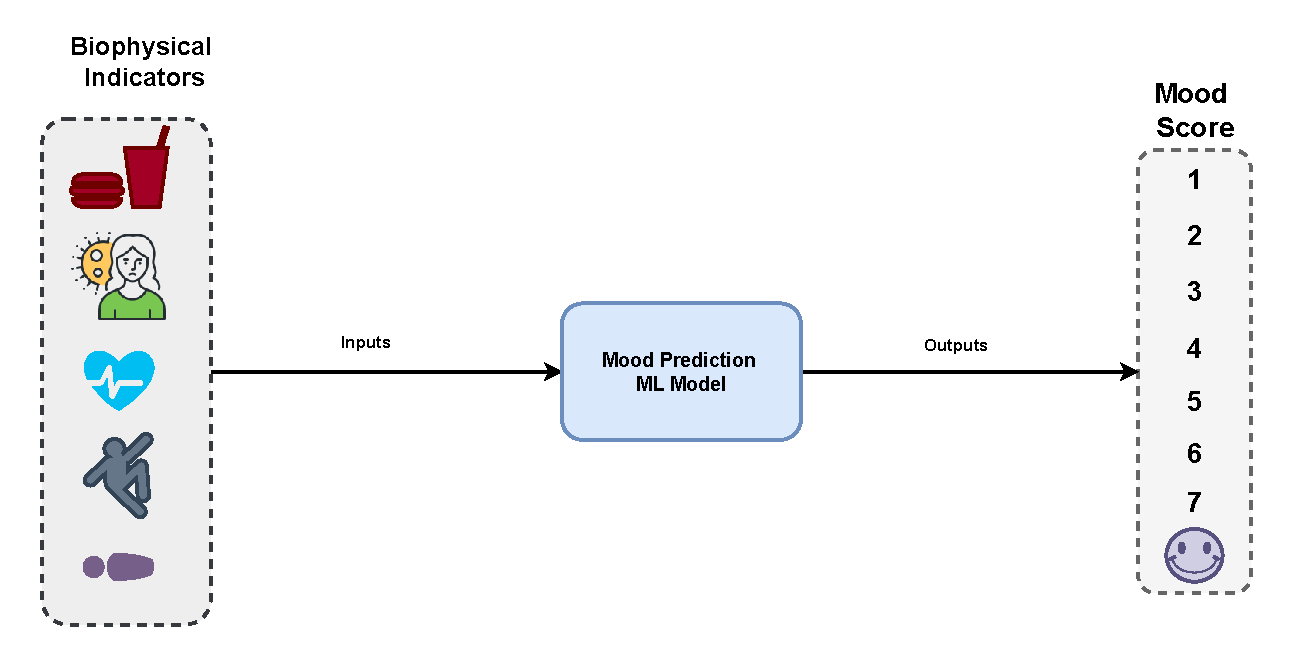
\includegraphics[width=\textwidth]{lit_review/fig/ML_Pipeline.pdf}
  \caption{The general ML methodology for mood score prediction.}
  \label{fig:ml_pipeline}
\end{figure}

Therefore, interest has grown towards approaches that supplement clinical interventions. Studies have shown that lifestyle interventions, such as better sleep hygiene \cite{carney_cognitive_2017}, practising mindfulness \cite{ramel1_effects_2004}, physical activity interventions \cite{andersson_physical_2015}, and dietary interventions \cite{opie_modified_2018, parletta_mediterranean-style_2019, liu_low_2017}, have promise in managing depression \cite{sarris_lifestyle_2014}. Given the prevalence of devices with sensors that can be used to monitor biophysical data, such as lifestyle activities using smartphones and smartwatches, researchers are proposing using such devices for detecting, monitoring and managing depression \cite{highland_review_2022}. The use of wearable technology to supplement clinical approaches is particularly appealing as it is unobtrusive, real-time, often passive (requiring little or no active input by a depressed individual/patient), of finer granularity (more data in the same time period) and allows assessments to occur in the person's usual environment \cite{ross_novel_2023}.

As changes in mood and consistently low mood are often associated with depression, studies have tried to use mood as an indicator to monitor and predict the progression of depression. Previous studies have used data from a variety of sensors on these devices, such as GPS location \cite{canzian_trajectories_2015, dogrucu_moodable_2020, xu_leveraging_2021}, phone and app usage patterns \cite{chiu_multimodal_2021, nadeem_depression_2022, mastoras_touchscreen_2019}, voice and ambient noise \cite{niu_time-frequency_2021}, and motion sensor information \cite{ghandeharioun_objective_2017}, to either detect or predict future changes in mood. These studies have focused primarily on using Machine Learning (ML) and its subtype, Deep Learning (DL), models to develop predictive models owing to their excellent ability to learn associations in complex data (see Figure \ref{fig:ml_pipeline} for a general methodology). Moreover, other studies categorise the sensor data into activity data, sleep data, heart data or phone usage data and then build ML- and DL-based predictive models using them \cite{choi_depressed_2022, ghandeharioun_objective_2017, nguyen_deep_2021, moshe_predicting_2021, little_deep_2021, thakre_polysomnographic_2022, tazawa_evaluating_2020, coutts_deep_2020}.

However, most previous studies using ML- and DL-based predictive models have focused on cross-sectional research, despite the failure of cross-sectional studies to apply to larger, more representative samples \cite{muller_depression_2021}. Moreover, cross-sectional works fail to account for the substantial inter-individual variability in clinical response to the same treatment or behavioural recommendations for depression due to genetic, environmental, behavioural, lifestyle, and interpersonal risk factors \cite{belmaker_major_2008, drysdale_resting-state_2017}. Personalised models built on longitudinal data are more suited to account for such variability. Hence, recent works have begun focusing on personalised, predictive models for depression \cite{choi_depressed_2022, xu_leveraging_2021, kathan_personalised_2022, jacobson_passive_2020, shah_personalized_2021}. 

Nevertheless, these studies have used monolithic ML models, which are not only large but also not properly explainable due to their large number of features and their interdependence. Using post-hoc explainability methods only extracts the most influential features/inputs of the model, which is not enough to explain the mood score, leading to a lack of trust in the model. The use of compositional ANN models can not only help improve model performance by learning better representations from biophysical data, but it can also address issues of explainability by decomposing the model into smaller, more explainable components.




\section{Summary}

This chapter reviewed literature on compositional \gls{ml} for \glspl{cps}. We first distinguished model-level decomposition of a single \gls{ann} from system-level pipeline composition in autonomous driving, and identified the lack of systematic, quantitative studies comparing monolithic and compositional \gls{ann} designs. We then surveyed work on \gls{fpga}-based \gls{ann} implementation, compositional verification and runtime enforcement, and compositional explainability, noting in each area that existing methods treat models as monolithic black boxes or compose only at the system level. Finally, we reviewed the \gls{av} and depression case-study literatures, where monolithic models dominate despite safety, timing, and interpretability requirements that align with a compositional approach. Together, these strands motivate the technical contributions developed in the remainder of the thesis.

